\documentclass{rapport}
\usepackage{lipsum}
\usepackage{gensymb}
\usepackage{float}
\usepackage{graphicx} % Required for inserting images

\usepackage{multirow}
\usepackage{enumerate}
\usepackage[shortlabels]{enumitem}
\usepackage{amsmath}
\usepackage{nomencl} % For nomenclature and acronyms
\makenomenclature % Activate nomenclature

\title{Cryptanalysis - Biclique Attack Report} %title of the file

\begin{document}

%----------- Report information ---------

\logo{logos/ULB_round.png}
\uni{\textbf{Université Libre de Bruxelles}}
\ttitle{Biclique Attack on AES-128} %title of the file
\subject{INFO-F-537: Cryptanalysis} % Subject name
\topic{Project Report} % Topic name

\professor{Prof. \textsc{Van Assche} Gilles} % information related to the professor

\students{\textsc{Amanor} Deborah\\
          \textsc{Hassani} Mortaza} % information related to the students

%----------- Init -------------------

\buildmargins % display margins
\buildcover % create the front cover of the document
\toc % creates the table of contents

%------------ Report body ----------------

\section{Introduction}
The \textbf{biclique attack} is an advanced variant of the \textbf{Meet-in-the-Middle} (MITM)\nomenclature{MITM}{Meet-in-the-Middle} attack, for the cryptanalysis of block ciphers to recover secret keys. It addresses the limitations of the traditional MITM attack, which is limited in breaking ciphers without independent key bits. In a biclique attack, the process begins by partitioning all possible secret keys into groups. For each group, a biclique structure is constructed. This structure helps in filtering out incorrect keys through partial matching, leaving candidate keys. A valid \emph{plaintext-ciphertext pair (P, C)} is used to determine the correct key. Since biclique cryptanalysis is based on MITM attacks, it is applicable to most block ciphers. In this report, we will focus on the biclique attack applied to the full AES block cipher. 

\nomenclature{AES}{Advanced Encryption System}AES has been one of the most widely used and trusted block ciphers for decades. Despite several cryptanalysis efforts, no significant progress has been made in recovering the secret key of the full round AES with a computational complexity less than exhaustive key search. This is because AES was designed to withstand differential and linear cryptanalysis. (reference paper) 

Impossible Differential Cryptanalysis was the first method to successfully attack a reduced version of AES, specifically targeting 7 rounds of AES-128. Similarly, the Square Attack was able to break 8 rounds of AES-192. These attacks, however, have not been able to extend to the full rounds of AES. 

Currently, the only attack known to break the full rounds of AES faster than exhaustive key search is the biclique attack, introduced in 2011 by Bogdanov et al(reference). This attack represented a breakthrough in cryptanalysis of the AES block cipher by achieving key recovery of the full rounds with the following reduced computational complexities: 

\begin{table}[h!]
    \centering
    \begin{tabular}{|p{3cm}|p{3cm}|p{3cm}|}
        \hline
        \multicolumn{3}{|c|}{Computation Operations} \\
        \hline
        AES & Brute Force & Biclique \\
        \hline
        128 & $2^{128}$ & $2^{126.18}$ \\
        \hline
        192 & $2^{192}$ & $2^{189.74}$ \\
        \hline
        256 & $2^{256}$ & $2^{254.42}$ \\
        \hline
    \end{tabular}
    \caption{Biclique key recovery for AES}
    \label{table:1}
\end{table}
% \begin{itemize}
%     \item     AES-128: 2\textsuperscript{126.18}  operations
%     \item     AES-192: 2\textsuperscript{189.74}  operations  
%     \item     AES-256 and 2\textsuperscript{254.42} operations
% \end{itemize}

While biclique cryptanalysis breaks the full AES, this is a theoretical attack and does not pose a practical threat due to its high computational complexity. In this report, we provide a detailed explanation of: 
\begin{enumerate}
    \item     The concept and construction of Bicliques 
    \item     The general Biclique Attack 
    \item     The application of the Biclique attack on AES block cipher 
    \item     An implementation of the attack on a reduced version of AES. 
\end{enumerate}

\newpage
\section{Background}
The concept of bicliques was first introduced in the cryptanalysis of hash functions. It originates from the \emph{splice-and-cut} framework in hash function cryptanalysis, more specifically its element called initial structure. The biclique approach led to the best preimage attacks on the SHA family of hash functions so far, including the attack on 50 rounds of SHA-512, and the first attack on a round-reduced Skein hash function. (paper) 

 

The biclique attack is a variant of the \emph{meet-in-the-middle} (MITM) attack. 
It utilizes a biclique structure to extend the number of rounds that can be attacked compared to the basic MITM attack. 
In mathematics, a biclique is a special type of \textbf{bipartite graph} where every vertex of the first set is connected to every vertex of the second set. (wikepedia). 
It can be denoted as \(K_{mn}\), where $m$ is the number of vertices in the first set and $n$ is the number of vertices in the second set. 

\begin{figure}[h]
    \centering
    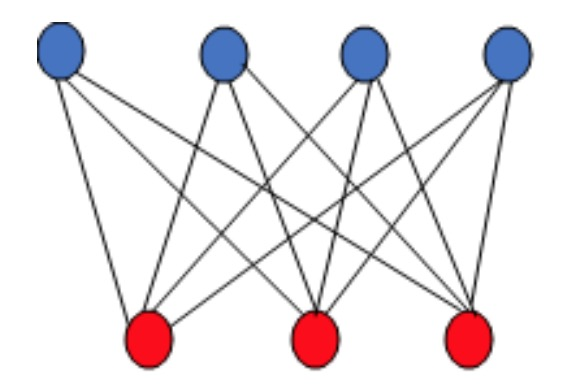
\includegraphics[width=0.25\textwidth]{figures/1.jpg}
    \caption{biclique with m=4 and n=3}
    \label{fig:biclique with m=4 and n=3}
\end{figure}
% \nomenclature{ABC}{Abbreviation Example}

Since the biclique attack builds on the principles of the MITM attack, we briefly describe the basic MITM attack to provide foundational context. 

\subsection{The Basic MITM}
The MITM attack is a time-memory trade of attack which is applied on block ciphers with independent key bits. This means that the keys used for encryption and decryption do not rely on each other, making block ciphers with multiple encryption rounds, such as double \nomenclature{DES}{Data Encryption Standard}DES (2DES), particularly vulnerable. For instance, in double DES, with a key size of $2^{112}$, MITM reduces the computational complexity of recovering the key from $2^{112}$ by using exhaustive key search to $2^{57}$. 

However, due to the key scheduling and subkey dependencies of AES, where keys for different rounds are derived from each other, MITM is not effective. And as such, the number of AES rounds that can be broken using this technique is relatively small. 

For a block cipher with a key size $2^n$, an adversary partitions the key space into groups of size $2^{\text{d}} \times 2^{\text{d}}$, where \(n = 2d\). The keys are represented as a matrix \(K[i, j]\), and the cipher is divided into two sub-ciphers: $g_1$ representing the forward computation and $g_2$ backward computation. 
\subsubsection{Steps in the MITM Attack }
\begin{enumerate}
    \item \textbf{Forward Computation} The adversary encrypts the known plaintext $P$ using all possible values of the first key subset $2^d$. The intermediate values $V_{i}$ are computed and stored alongside the corresponding key values
    \\
    \begin{equation}
        g_1 = ENC_{k_1}(p)
    \end{equation}

    \begin{equation}
        P \xrightarrow[\quad g_1 \quad]{K[i, \cdot]} v_i
    \end{equation}

    \item 	\textbf{Backward Computation} The adversary decrypts the known ciphertext using all possible values of the second key subset $2^{d}$. The Intermediate values $V_j$ are computed and stored alongside their respective keys
        \begin{equation}
            g_2 = DEC_{k_2}(C)
        \end{equation}

        \begin{equation}
            v_j \xleftarrow[\quad g_2 \quad]{K[\cdot, j]} C
        \end{equation}


    \item	\textbf{Matching} The adversary compares the intermediate values, $V_{i}$  and $V_{j}$ to find a match. If \(V_i = V_j\) , then \(K[i, j]\) are the candidate key pairs

\end{enumerate}
The basic meet-in-the-middle attack has clear limitations in AES cipher cryptanalysis since an intermediate value can be found for a very small number of rounds only. Biclique cryptanalysis overcomes these limitations by introducing a more advanced structure, enabling attacks on the full AES.

\section{The Biclique Attack}
A \textbf{biclique} is a mathematical structure used in cryptanalysis of block ciphers to efficiently explore relationships between keys, plaintexts, and ciphertexts in a cipher. It connects $2^d$ intermediate states $\{S_j\}$ to $2^d$ Ciphertexts $\{C_i\}$ using $2^{2d}$ keys represented as $K[i, j]$. Each key $K[i, j]$ maps an intermediate state $\{S_j\}$ to a ciphertext $\{C_i\}$ through a subcipher $f$, mathematically expressed as:
\begin{equation}
    \forall i, j : S_j \xrightarrow[\quad f \quad]{K[i, j]} C_i
\end{equation}


\begin{equation}
C_i = f_{K[i, j]}(S_j), \forall i, j \in \{0, \ldots, 2^d - 1\}
\end{equation}
A biclique is then said to be d-dimensional if it connects $2^d$ intermediate states to $2^d$ ciphertexts. The dimension d determines the size and complexity of the structure. 

\subsection{Preliminary Steps}
To conduct the attack, the adversary performs two preparatory steps; Key partitioning and Cipher splitting.

\begin{enumerate}
    \item \textbf{Key Partitioning:}
    The adversary firstly partitions the key space of the cipher into subsets or groups of size $2^{2d}$ for some $d$, where the keys are represented as $K[i, j]$ in a matrix $2^d \times 2^d$ similar to that of the MITM.

    \item \textbf{Cipher splitting}
    The adversary then splits the cipher into two subciphers, $f$ and $g$ such that the encryption process $e$ can be expressed as:
    
    \begin{equation}
        e = f \circ g
    \end{equation}
    
\end{enumerate}
Where $g$ maps the plaintext $P$ to an intermediate state $S$, and $f$ maps the intermediate state $S$ to the ciphertext $C$.


\subsection{Constructing bicliques}
After executing the preliminary steps, the next step is to construct the biclique.

\subsubsection{Naïve Approach or Bruteforce}
A straightforward way to construct the biclique is to use the naive approach or brute-force method. This can be achieved when the adversary maps $2^d$ intermediate states to $2^d$ ciphertexts and then derives a key $K[i, j]$ for each intermediate state-ciphertext pair shown in eqn 5. However, this involves evaluating the cipher for all $2^{2d}$ possible key pairs thus increasing the computational complexity because it takes a lot of time. A much more efficient way is for the adversary to choose the keys in advance and require them to conform to specific differentials:

\subsubsection{Independent Related Key Differentials}
This approach exploits differences in keys and how they propagate through the cipher. In this case, two types of differentials are used over the subcipher $f$, $\Delta_i$-differentials and $\nabla_j$-differentials.

\begin{itemize}
    \item $\Delta_i$-differentials: shows a difference in the output $\Delta i$ under a key difference $\Delta K_i$ when there is no difference in the starting state. This means that a specific difference in the key ($\Delta K_i$) produces a predictable difference ($\Delta$) in the ciphertext:
    
    \begin{equation}
        0 \xrightarrow[\quad f \quad]{\Delta^K_i} \Delta_i
    \end{equation}

    \item $\nabla_j$-differentials: A difference in the input $\nabla j$ and the key $\nabla K_j$ reveals no difference in the output ciphertext:

    \begin{equation}
        \nabla_j \xrightarrow[\quad f \quad]{\nabla^K_j} 0
    \end{equation}

\end{itemize}

To construct the biclique, a base key \( K[0,0] \) is chosen which maps the intermediate states \( S_0 \) to the ciphertext \( C_0 \) over the subcipher \( f \).

 \begin{equation}
    C_0 = f_{K[0,0]}(S_0) 
 \end{equation}

 The two sets of related-key differentials \( \Delta K_i \) and \( \nabla K_j \) are combined by an XOR operation only if the trails of \( \Delta_i \)-differentials do not share active non-linear components such as S-boxes with the trails of \( \nabla_j \)-differentials. Thus we obtain a \( 2^d \times 2^d \) matrix of the keys i.e \( (\Delta_i, \nabla_j) \):

\begin{equation}    
     \nabla_j \xrightarrow[\substack{f }]{\Delta_i^K \oplus \nabla_j^K} \Delta_i \text{ for } i, j \in \{0, \ldots, 2^d - 1\}.
\end{equation}

If the trails of the differentials do not share any active non-linear components, the differentials are completely independent and can be directly combined. The result is combined with the base key, \( K[0,0] \) and initial intermediate state \( S_0 \), ciphertext pair \( C_0 \).

 \begin{equation}
    S_0 \oplus \nabla_j \xrightarrow[\substack{f }]{K[0,0] \oplus \Delta_i^K \oplus \nabla_j^K} C_0 \oplus \Delta_i.
 \end{equation} 
 The result is a biclique where the subsequent intermediate states, ciphertext and keys can be obtained by:

 \begin{equation}
    \begin{aligned}
        S_j &= S_0 \oplus \nabla_j, \\
        C_i &= C_0 \oplus \Delta_i, \text{ and} \\
        K[i, j] &= K[0, 0] \oplus \Delta_i^K \oplus \nabla_j^K.
    \end{aligned}
 \end{equation}

 This construction satisfies the biclique condition where every key \( K[i,j] \) maps an intermediate state \( S_j \) to a ciphertext \( C_i \) and get a \( d \)-dimensional biclique. The independence of the related-key differentials ensures that the biclique can be efficiently constructed with computational complexity of \( 2 \cdot 2^d \) evaluations of the subcipher \( f \), instead of \( 2^{2d} \) that the naive approach provides.

 \subsection{Steps of the General Biclique Attack}

 After successful preparation, the adversary moves on to implement the attack in the following steps;

 \begin{enumerate}[start = 1, label={(\bfseries Step\arabic*):}]
    \item \textbf{Constructing the Biclique} For each group of keys, \( K[i, j] \), the adversary constructs a biclique structure which maps \( 2^d \) intermediate states \( \{S_j\} \) to \( 2^d \) ciphertexts \( \{C_i\} \). This structure is based on what was discussed in the section \textit{Constructing bicliques}.
            \begin{equation}
                \begin{array}{ccc}
                    S_0 & K[0,0] & C_0 \\
                    \vdots & \vdots & \vdots \\
                    S_{2^d-1} & K[2^d-1,2^d-1] & C_{2^d-1}
                    \end{array}
            \end{equation}
                
            \begin{equation}
                \forall i, j : S_j \xrightarrow[\quad f \quad]{K[i, j]} C_i
            \end{equation}

    \item \textbf{Obtain the data} The adversary takes the possible ciphertexts $C_i$ and passes it through the decryption oracle. With the secret key $K_{\text{secret}}$ unknown to the adversary, the oracle decrypts the ciphertext $C_i$ and returns the corresponding set of $2^d$ plaintexts.
            \begin{equation}
                C_i \xrightarrow[\epsilon^{-1}]{\text{decryption oracle}} P_i.
            \end{equation}
    \item \textbf{Meet-In-The-Middle} For each key $K[i, j]$ in the group, the adversary maps the plaintexts obtained in step 2 to their respective intermediate state $S_j$ the using the first subcipher $g$. Simultaneously, the adversary computes the \textbf{ciphertexts} backward to their intermediate states $S_j$ using the second subcipher $f$. Using the MITM approach, the adversary tries to match the forward and backward computations at the intermediate state $S_j$ .
            \begin{equation}
                \exists i, j : P_i \xrightarrow[g]{K[i, j]} S_j.
            \end{equation}
    \item \textbf{Matching with Precomputations} For each key candidate, $K[i, j]$, the adversary evaluates the cipher directly to check if the computed intermediate states and ciphertexts match the expected results for the given plaintext-ciphertext pair. A valid pair proposes $K[i, j]$ as a key candidate.


 \end{enumerate}

 \subsubsection{Improvement with Precomputation}
 The matching process in step 4 can be significantly improved with precomputations.The adversary precomputes and stores in memory the partial results for the forward and backward computations:

 \begin{itemize}
    \item \textbf{Forward computation:} Compute the intermediate states $S_j$ for all possible plaintexts $P_i$ using a fixed key $K[i, 0]$.
    \item \textbf{Backward computation:} Compute the intermediate states $S_j$ for all ciphertexts $C_i$ using a fixed key $K[0, j]$.
 \end{itemize}

 \begin{equation}
    \text{for all } i \quad P_i \xrightarrow{K[i, 0]} \vec{v} \quad \text{and} \quad \text{for all } j \quad \vec{v} \xleftarrow{K[0, j]} S_j
 \end{equation}
 Instead of recalculating all intermediate states for each key $K[i, j]$ from scratch, the adversary \textbf{recomputes only the parts of the cipher that differ} from the precomputed results. The amount of recalculation depends on the diffusion properties of both internal rounds and the key schedule of the cipher. This approach significantly reduces the number of operations compared to what was presented in (step 4).


 \section{Biclique Attack on the Full AES-128 Cipher}

 \subsection{Brief Description of AES-128}

 \section{Reduced Implementation of the Attack on AES}
\end{document}
